\section{Problem 2 - Topology}
\textit{Consider the overhearing topology studied in the Network Coding Lecture. Assume initially no losses in the links and think of the number of transmissions and reception operations that each of the nodes performs, using the activity diagrams from the previous exercises. Is the relay acting selfishly when network coding is used ? Are the sources acting in their best interest (both transmitting and receiving incur a cost)}
\begin{figure}[!h]
  \centering
  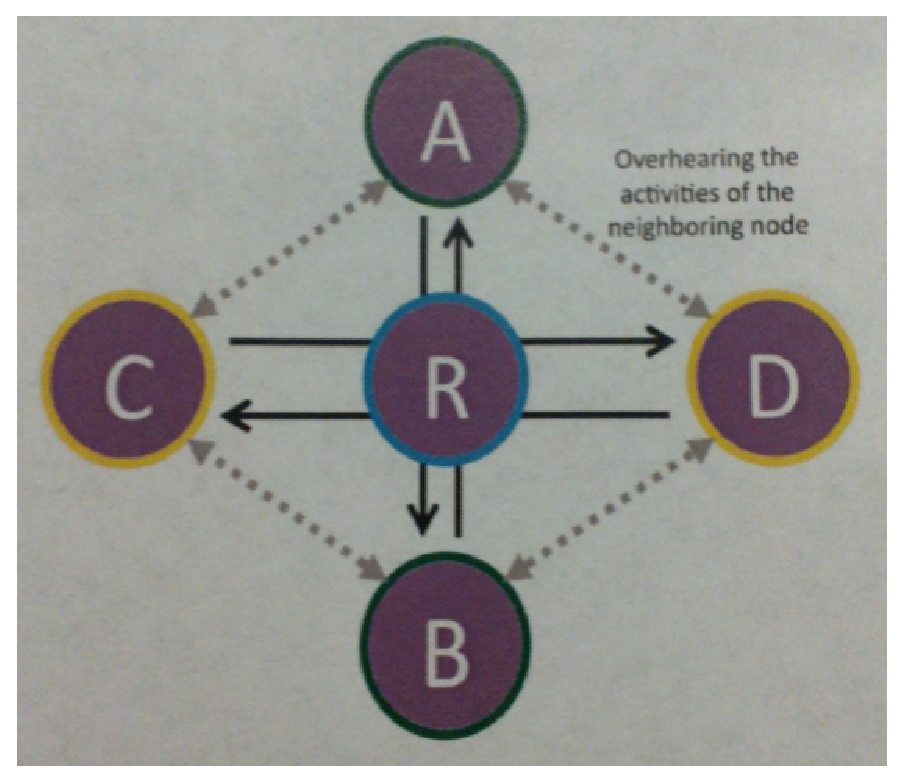
\includegraphics[width=6cm]{MM10_thecross.eps}
  \caption{The butterfly cross (aka. the only fig. you need for network coding)}
  \label{fig:MM10_thecross}
\end{figure}

If one where to imaging a perfect world then a cooperation strategy would benefit all. If however one where to think about the cost, in for instance power, the relay would have to pay then many scenarios could be imagined where the relay is the loser of the system. If the nodes where semi stationary then one node (having good connections) would always be helping the others with little in return. If however the nodes is very mobile the averaging effect of being in good and bad conditions levels out the benefit for all. One could also have a scenario where one node is low on battery and would like to save as much as possible and therefore must act selfishly in order to obtain this. Applying network coding decreasing the amount of transmissions needed by the relay will, if assumed that the relay have to operate, be selfish by the relay in the sense that it saves power with the cost of perhaps slowing down communication between the two other nodes.